\section{Observation and Calculations}

\subsection{Estimation of operating voltage of the Scintillation Detector}
We have obtained the count vs. LLD voltage plots for different values of operating high voltage. The resolution for a particular operating voltage is defined as the ratio of the FWHM of the distribution and the peak count value. It can be observed that the resolution varies with the applied voltage and the voltage at which we get the best resolution is fixed as the operating voltage for the rest of the experiment.

Table \ref{tab:ov} details the V versus count data at different operating voltages. Figs. \ref{450} to \ref{650} plot the V versus count data to a Gaussian fit and Table \ref{tab:resolution} summarises the estimation of ideal operating voltage from the resolutions. 

\begin{table}[]
    \centering
    % \resizebox{\columnwidth}{!}{%
    \begin{tabular}{|c|ccccc|}
    \hline
    \multirow{2}{*}{LLD (V)} & \multicolumn{5}{c|}{Counts at different Operating Voltages} \\ \cline{2-6} 
     & \multicolumn{1}{c|}{450V} & \multicolumn{1}{c|}{500V} & \multicolumn{1}{c|}{550V} & \multicolumn{1}{c|}{600V} & 650V \\ \hline
    2.4 & \multicolumn{1}{c|}{1688} & \multicolumn{1}{c|}{1084} & \multicolumn{1}{c|}{-} & \multicolumn{1}{c|}{-} & 1282 \\ \hline
    2.5 & \multicolumn{1}{c|}{1794} & \multicolumn{1}{c|}{1181} & \multicolumn{1}{c|}{-} & \multicolumn{1}{c|}{-} & 1575 \\ \hline
    2.6 & \multicolumn{1}{c|}{1801} & \multicolumn{1}{c|}{1096} & \multicolumn{1}{c|}{-} & \multicolumn{1}{c|}{-} & 2163 \\ \hline
    2.7 & \multicolumn{1}{c|}{1959} & \multicolumn{1}{c|}{1055} & \multicolumn{1}{c|}{2897} & \multicolumn{1}{c|}{2083} & 4028 \\ \hline
    2.8 & \multicolumn{1}{c|}{2112} & \multicolumn{1}{c|}{1096} & \multicolumn{1}{c|}{4153} & \multicolumn{1}{c|}{2912} & 7715 \\ \hline
    2.9 & \multicolumn{1}{c|}{2194} & \multicolumn{1}{c|}{2008} & \multicolumn{1}{c|}{7871} & \multicolumn{1}{c|}{4914} & 9342 \\ \hline
    3 & \multicolumn{1}{c|}{2275} & \multicolumn{1}{c|}{8220} & \multicolumn{1}{c|}{10203} & \multicolumn{1}{c|}{9417} & 9167 \\ \hline
    3.1 & \multicolumn{1}{c|}{2146} & \multicolumn{1}{c|}{11619} & \multicolumn{1}{c|}{8135} & \multicolumn{1}{c|}{11449} & 7286 \\ \hline
    3.2 & \multicolumn{1}{c|}{2094} & \multicolumn{1}{c|}{9304} & \multicolumn{1}{c|}{6475} & \multicolumn{1}{c|}{8943} & 6473 \\ \hline
    3.3 & \multicolumn{1}{c|}{1913} & \multicolumn{1}{c|}{4464} & \multicolumn{1}{c|}{5378} & \multicolumn{1}{c|}{7096} & 5450 \\ \hline
    3.4 & \multicolumn{1}{c|}{1799} & \multicolumn{1}{c|}{1642} & \multicolumn{1}{c|}{4437} & \multicolumn{1}{c|}{5931} & 4457 \\ \hline
    3.5 & \multicolumn{1}{c|}{-} & \multicolumn{1}{c|}{-} & \multicolumn{1}{c|}{-} & \multicolumn{1}{c|}{4782} & 3154 \\ \hline
    3.7 & \multicolumn{1}{c|}{-} & \multicolumn{1}{c|}{-} & \multicolumn{1}{c|}{-} & \multicolumn{1}{c|}{4093} & 2120 \\ \hline
    3.8 & \multicolumn{1}{c|}{-} & \multicolumn{1}{c|}{-} & \multicolumn{1}{c|}{-} & \multicolumn{1}{c|}{3569} & 1147 \\ \hline
    \end{tabular}%
    % }
    \caption{LLD vs. Count data for Cs-137 at different operating voltages}
    \label{tab:ov}
    \end{table}

\begin{figure}[H]
    \centering
    \includegraphics[width=1\columnwidth]{images/450.eps}
    \caption{Cs-137 photopeak spectrum at 450V}
    \label{450}
\end{figure}

\begin{figure}[H]
    \centering
    \includegraphics[width=0.9\columnwidth]{images/500.eps}
    \caption{Cs-137 photopeak spectrum at 500V}
    \label{500}
\end{figure}

\begin{figure}[H]
    \centering
    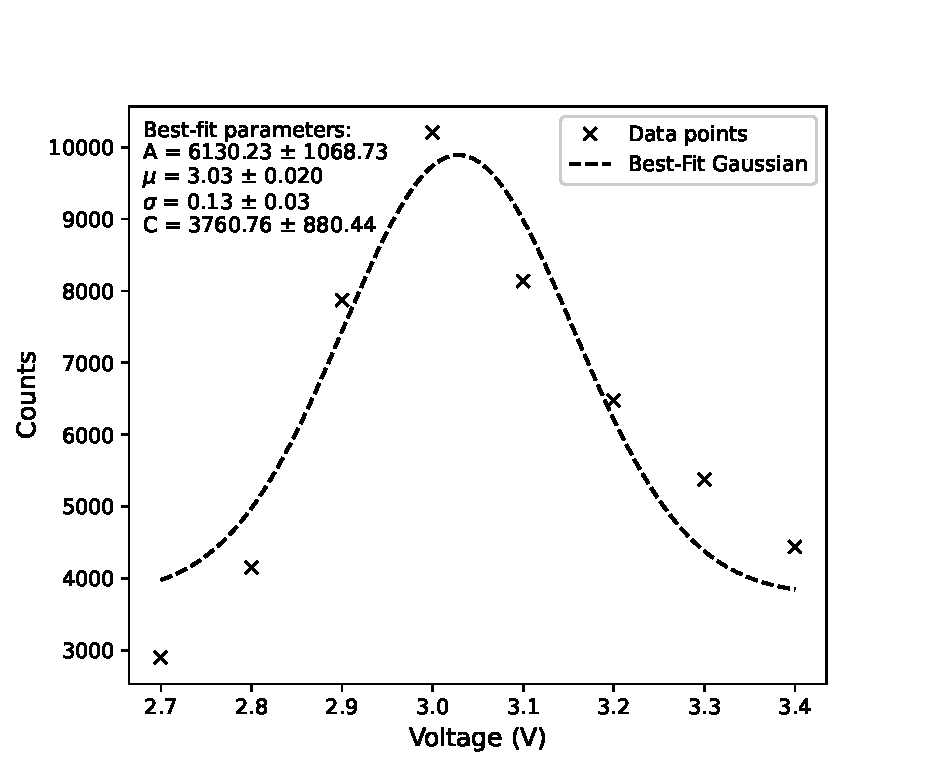
\includegraphics[width=0.9\columnwidth]{images/550.eps}
    \caption{Cs-137 photopeak spectrum at 550V}
    \label{550}
\end{figure}

\begin{figure}[H]
    \centering
    \includegraphics[width=0.9\columnwidth]{images/600.eps}
    \caption{Cs-137 photopeak spectrum at 600V}
    \label{600}
\end{figure}

\begin{figure}[H]
    \centering
    \includegraphics[width=0.9\columnwidth]{images/650.eps}
    \caption{Cs-137 photopeak spectrum at 650V}
    \label{650}
\end{figure}

\begin{figure}[H]
    \centering
    \includegraphics[width=1\columnwidth]{images/ov.eps}
    \caption{Applied voltage vs. resolution characterstics}
    \label{ov}
\end{figure}

\begin{table}[H]
    \centering
    \begin{tabular}{|c|c|c|c|}
    \hline
        Operating Volt. & Max. Height at (V) & FMWH & Resolution (\%) \\ \hline
        450 & 2.99 & 0.57 & 19.02 \\ \hline
        500 & 3.11 & 0.28 & 9.14 \\ \hline
        550 & 3.02 & 0.30 & 9.86 \\ \hline
        600 & 3.13 & 0.34 & 11.02 \\ \hline
        650 & 3.12 & 0.34 & 19.26 \\ \hline
    \end{tabular}
    \caption{Operating voltage vs FMWH and resolution}
    \label{tab:resolution}
\end{table}

Hence from Fig. \ref{ov}, we have the best operating voltage for the setup as 500V with a resolution of 9.14\%.

\subsection{Study of Cs-137 spectrum using SCA}

Now, fixing the SCA setup at the operating voltage, we took V vs count data for Cs-137. The values are given in Table \ref{tab:cs137} and plotted in Fig. \ref{cs137}.

\begin{table}[H]
    \centering
    \begin{tabular}{|c|c|c|c|}
    \hline
    LLD (V) & Count & LLD (V) & Count \\ \hline
    1 & 3560 & 2.3 & 1127 \\ \hline
    1.1 & 2881 & 2.4 & 954 \\ \hline
    1.2 & 2564 & 2.5 & 915 \\ \hline
    1.3 & 2414 & 2.6 & 1134 \\ \hline
    1.4 & 2332 & 2.7 & 2471 \\ \hline
    1.5 & 2338 & 2.8 & 7688 \\ \hline
    1.6 & 2187 & 2.9 & 11254 \\ \hline
    1.7 & 2209 & 3 & 6572 \\ \hline
    1.8 & 2207 & 3.1 & 2265 \\ \hline
    1.9 & 2189 & 3.2 & 690 \\ \hline
    2 & 2077 & 3.3 & 223 \\ \hline
    2.1 & 1761 & 3.4 & 135 \\ \hline
    2.2 & 1452 & 3.5 & 92 \\ \hline
    \end{tabular}
    \caption{LLD vs. Count data for Cs-137 at an operating voltage of 500V}
    \label{tab:cs137}
    \end{table}

\begin{figure}[H]
    \centering
    \includegraphics[width=1\columnwidth]{images/cs137.eps}
    \caption{Energy Spectrum of Cs-137}
    \label{cs137}
\end{figure}

In Fig. \ref{cs137}, using the photopeak at 662 keV, the resolution of the detector can be calculated from the FWHM and the $\mu$ value as, $\boxed{8.37\%}$.

\subsection{Study of Co-60 and Cs-137 spectra using MCA}

Fig. \ref{espec} shows the energy spectra of Cs-137 and Co-60 analysed my the MCA.

\begin{figure}[H]
    % \ContinuedFloat
    % \bigskip
    \begin{subfigure}{\linewidth}
    \includegraphics[width=1\textwidth]{images/co60.png}
    \caption{Co-60}
    \end{subfigure}
    
    % \bigskip
    \begin{subfigure}{\linewidth}
    \includegraphics[width=1\textwidth]{images/cs137.png}
    \caption{Cs-137}
    \end{subfigure}
    \caption{Plots showing the Energy Spectrum analysed using MCA}
    \label{espec}
\end{figure}

The details of the analysis are presented in Tables \ref{tab:mca1} and \ref{tab:mca2}.

\begin{table}[H]
    \centering
    \begin{tabular}{|c|c|}
        \hline
        \textbf{Start}           & 269      \\ \hline
        \textbf{End}             & 337      \\ \hline
        \textbf{Peak}            & 304.9182 \\ \hline
        \textbf{TM/HM}           & 1.7814   \\ \hline
        \textbf{FMHM}           & 28.0935   \\ \hline
        \textbf{Gross}           & 61475    \\ \hline
        \textbf{Net}             & 54885.5  \\ \hline
    \end{tabular}
    \caption{Cs-137 Peak Report}
    \label{tab:mca1}
\end{table}

\begin{table}[H]
    \centering
    \begin{tabular}{|c|c|c|}
        \hline
        & Peak 1    &   Peak 2 \\ \hline
        \textbf{Start}           & 566    &  490\\ \hline
        \textbf{End}             & 646  & 564   \\ \hline
        \textbf{Peak}            & 602.3283 & 530.2158 \\ \hline
        \textbf{TM/HM}           & 1.7433 & 1.5238  \\ \hline
        \textbf{FMHM}           & 34.2273 & 37.2411   \\ \hline
        \textbf{Gross}           & 18378 & 25152   \\ \hline
        \textbf{Net}             & 10116 & 12274  \\ \hline
    \end{tabular}
    \caption{Co-60 Peak Report}
    \label{tab:mca2}
\end{table}

From tables \ref{tab:mca1} and \ref{tab:mca2}, we can estimate the resolution of the detector as,

\begin{itemize}
    \item Cs-137: 9.21\%
    \item Co-60 (Peak 1): 5.68\%
    \item Co-60 (Peak 2): 7.02\%
\end{itemize}

\subsection{Energy Calibration of the spectrometer \& Estimation of Energy of an Sample Isotope}

Now, using the multiple channel analyser, three different sources were placed in front of detector at once and spectrum was analysed to obtain the calibration curve. The energy spectrum used were of Cs-137, Co-60 and Ba-133, whose photopeaks are known to us.

Fig. \ref{cal} shows the combined energy spectrum and table \ref{tab:cal} summarises the peaks shown in the figure.

\begin{figure}[H]
    \centering
    \includegraphics[width=1\columnwidth]{images/calibration.png}
    \caption{The combined energy spectrum of Cs-137, Co-60 and Ba-133, with four known peaks highlighted}
    \label{cal}
\end{figure}

\begin{table}[H]
    \centering
    \begin{tabular}{|c|c|c|c|}
    \hline
    I (A) & B (Gauss) & I (A) & B (Gauss)\\ \hline
    0 & 0 & 1.76 & 4920\\ \hline
    0.30 & 841 & 1.95 & 5410 \\ \hline
    0.55 & 1563 &2.27 & 5860\\ \hline
    0.72 & 2070 &2.51 & 6220\\ \hline
    0.99 & 2880 &2.71 & 6460\\ \hline
    1.28 & 3640 & 2.97 & 6740\\ \hline
    1.54 & 4380 &  & \\ \hline
    % 1.54 & 4380 &      & 
    \end{tabular}
    \caption{Calibration of magnetic field with current}
    \label{tab:cal}
\end{table}

\begin{figure}[H]
    \centering
    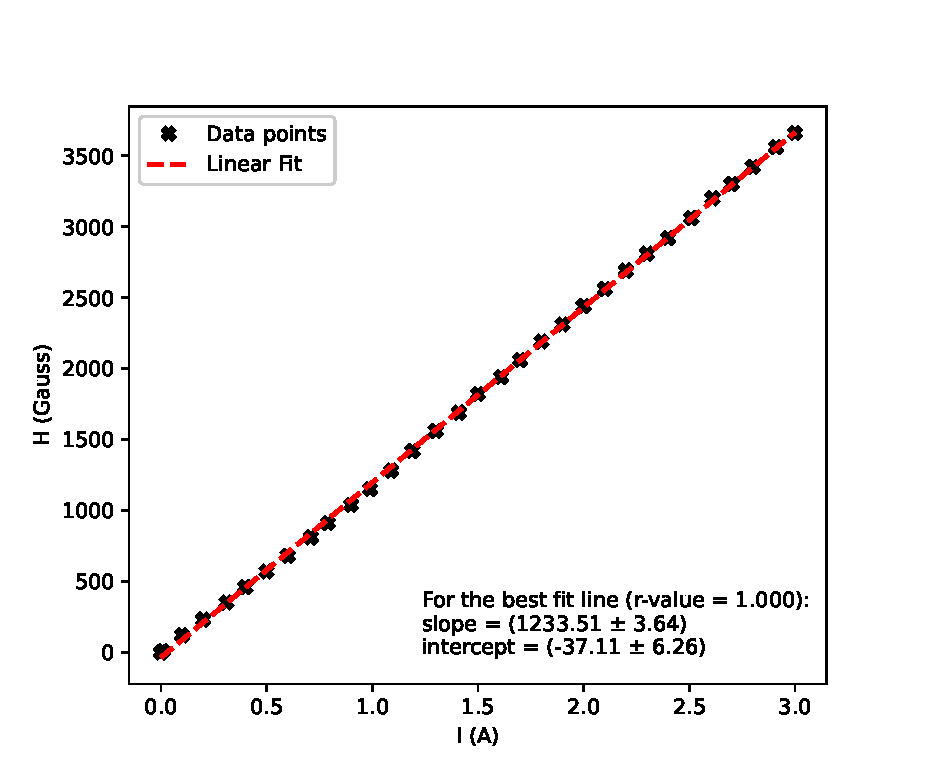
\includegraphics[width=1\columnwidth]{images/cal.eps}
    \caption{Calibration curve for the MCA}
    \label{calline}
\end{figure}

Fig. \ref{calline} shows the calibrated curve for the detector. Now we can analyse the energy spectrum of an unknown sample using this curve.

\subsubsection*{Analysis of an the energy spectrum of Na-22}

\begin{figure}[H]
    \centering
    \includegraphics[width=1\columnwidth]{images/na22.png}
    \caption{The energy spectrum of Na-22}
    \label{na22}
\end{figure}

Fig. \ref{na22} shows the energy spectrum of Na-22. Two peaks were detected at channels 238.1277 and 573.4547 respectively. Therefore, using the fit calibration curve obtained previously, the corresponding energy values are 511.80 keV and 1276.35 keV respectively.

\subsection{Estimation of the Mass Absorbance Coefficient of Aluminium}

For 662 keV gamma rays, the mass absorption coefficient of Al is measured by placing aluminum blocks of different thicknesses between the detector and the source. The net count (= total count $-$ background noise) as a function of thickness is presented in Table \ref{tab:al}.

\begin{table}[]
    \centering
    \begin{tabular}{|c|c|c|}
    \hline
    Thickness (cm) & Gross count & Net count \\ \hline
    0.0 & 28241 & 27187 \\ \hline
    0.5 & 25646 & 24592 \\ \hline
    1.0 & 23825 & 22771 \\ \hline
    1.5 & 21531 & 20477 \\ \hline
    2.0 & 19060 & 18006 \\ \hline
    2.5 & 17824 & 16770 \\ \hline
    3.0 & 15909 & 14855 \\ \hline
    3.5 & 14218 & 13164 \\ \hline
    4.0 & 13417 & 12363 \\ \hline
    4.5 & 11981 & 10927 \\ \hline
    5.0 & 10965 & 9911 \\ \hline
    5.5 & 9903 & 8849 \\ \hline
    6.0 & 9078 & 8024 \\ \hline
    \end{tabular}
    \caption{Net and gross counts around a fixed 662 keV peak with varying thicknesses of Al kept in front of the detector. Background count = 1054.}
    \label{tab:al}
    \end{table}

\begin{figure}[H]
    \centering
    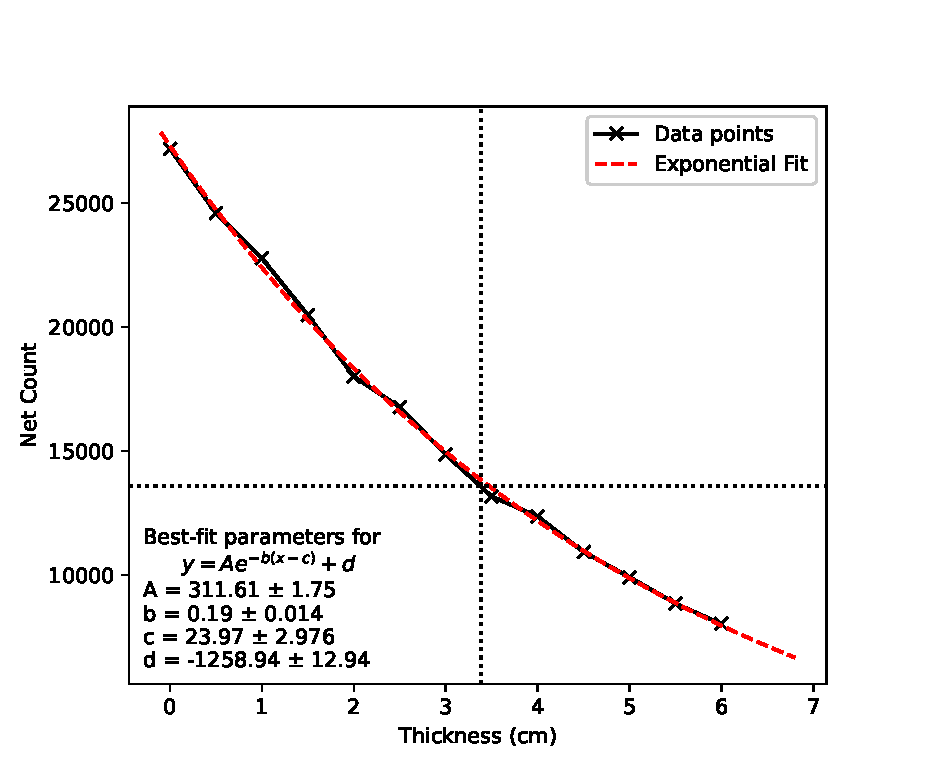
\includegraphics[width=1\columnwidth]{images/al.eps}
    \caption{Net count vs. thickness for aluminium. The dotted line highlights the half-value thickness at around 3.38cm}
    \label{al}
\end{figure}

From the graph Observed value of Half value thickness (thickness at which counts are reduced to half) is 3.38cm. This means density thickness $= 3.38\times 2.7 =9.13$ gm/cm$^2$ (using the density of aluminium). Hence, the mass absorption coefficient comes out to be,

\begin{align*}
    m=\frac{\ln(2)}{9.13} =0.076 \text{ gm/cm}^2
\end{align*}

\section{Error Analysis}

The error in a quantity $Q(a_1, a_2, ..., a_n)$ is calculated using,
\begin{align} \Delta Q &= \sqrt{\left( \sum_i^n \frac{\partial Q}{\partial a_i} \Delta a_i \right)^2} \end{align}

\subsubsection*{Resolution of the detector}
The uncertainity in resolution of the detector at the operating voltage can be calculated as from FWHM and the voltage at peak height, which comes out to be 0.92\%.

\subsubsection*{Peak energy values of Na-22}
The uncertainity in energy is directly a function of the uncertainities in the calibration curve. These values come out to be $(511.80 \pm 3.95)$ keV and $(1276.35 \pm 6.54)$ keV.

\subsubsection*{Mass Absorbance Coefficient of Al-22}
The uncertainity in $m$ is directly a related to the uncertainity in the estimation of HVT which is $0.5$ cm. Hence $\Delta m$ comes out to be $0.01$ gm/cm$^2$.